% !TEX root = article.tex

\ifdefined\noauthorea
\begin{figure}[t]
\begin{center}
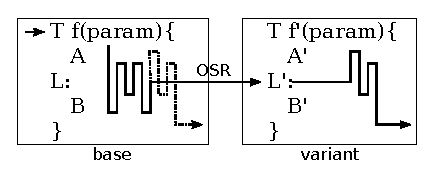
\includegraphics[width=0.6\columnwidth]{figures/overview-osr/overview-osr.eps}
\caption{\protect\label{fig:osr-dynamics} On-stack replacement dynamics: control is transferred via OSR from a point \textsf{L} of a base function \textsf{f} to a point \textsf{L'} in a variant \textsf{f'} of \textsf{f}.
  
  
  
  
  
  
  
  }
\end{center}
\end{figure}
\fi

\section{Approach}
\label{se:approach}

The key to platform independence in our approach is to encode the entire OSR machinery at intermediate representation level, without resorting to machine-level code manipulation.

\subsection{Overview}
\label{ss:overview}

Consider the generic OSR scenario shown in Figure~\ref{fi:osr-dynamics}. A base function \textsf{f} is executed and it can either terminate normally (dashed lines), or an OSR event may transfer control to a variant \textsf{f'}. The decision of whether an OSR should be fired at a given point \textsf{L} is based on an {\em OSR condition}. A typical example is a guard testing whether a function \textsf{f} has become unsafe and execution needs to fall back to a safe version \textsf{f'}. This scenario includes deoptimization of functions generated with aggressive speculative optimizations. Another example is a profile counter reaching a certain hotness threshold, which indicates that \textsf{f} is taking longer than expected and is worth optimizing. This is a frequent scenario in JIT-based virtual machines.

Classical OSR implementations adjust the stack so that execution can continue in \textsf{f'} with the current frame \mynote{add citations}. This requires manipulating the program at machine code level and is highly ABI- and compiler-dependent. A simpler approach, which we follow in this article, consists of creating a new frame every time an OSR is fired, essentially regarding an OSR transition as a function call \mynote{cite WebKit and McVM}. 

Our implementation targets two general scenarios: 1) {\bf resolved OSR}: \textsf{f'} is known before executing \textsf{f}, as in the deoptimization example discussed above; 2) {\bf open OSR}: \textsf{f'} is generated when the OSR is fired, supporting deferred compilation strategies. In both cases, for and OSR to be fired at a certain point \textsf{L}, the base function needs to be instrumented before its execution with code that checks the OSR condition. We denote with \textsf{f$_{OSRfrom}$} the OSR-instrumented version of \textsf{f}. If the condition is satisfied, control is transferred to \textsf{f'} via a function call. In the first scenario, shown in Figure~\ref{fi:overview-osr-final}, the OSR invokes an instrumented version of \textsf{f'}, which we call \textsf{f'$_{OSRto}$}. This is possible since \textsf{f'} is known when \textsf{f} is instrumented.

%and returns the same value when it has terminated. The assumption is that the called function produces the same side-effects and return values that one would obtain by \textsf{f} if no OSR were performed.

%\ref{fi:overview-osr-final}

%\begin{verbatim}
%int fac(int n) {
%    int i = 2, f = 1;
%    while (i<=n) f *= i++;
%    return f;
%}
%\end{verbatim}
%
%\begin{verbatim}
%int fac(int n) {
%    int i = 2, f = 1;
%    while (i<=n)  {
%        if (osr_cond) return fac_osr(n,i,f); 
%        f *= i++; 
%    } return f;
%}
%\end{verbatim}
%
%\begin{verbatim}
%int fac_osr(int n) {
%    goto L;
%    int i = 2, f = 1;
%    while (i<=n) L: f *= i++;
%    return f;
%}
%\end{verbatim}

\ifdefined\noauthorea
\begin{figure}[t]
\begin{center}
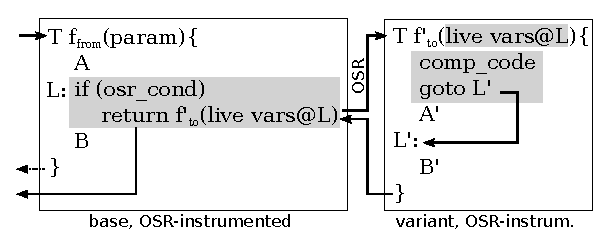
\includegraphics[width=0.7\columnwidth]{figures/overview-osr-final/overview-osr-final.eps}
\caption{\protect\label{fi:overview-osr-final} OSR-instrumented functions with resolved OSR call.}
\end{center}
\end{figure}
\fi

\ifdefined\noauthorea
\begin{figure}[t]
\begin{center}
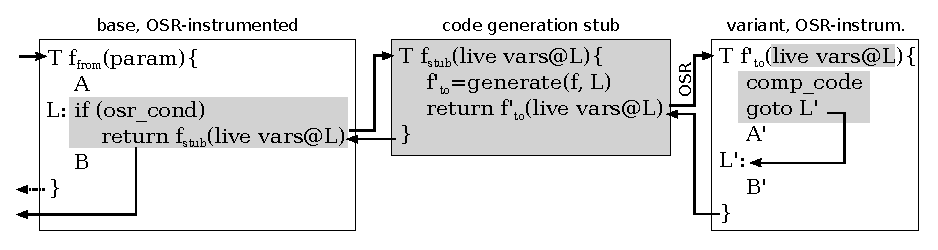
\includegraphics[width=1.0\columnwidth]{figures/overview-osr-open/overview-osr-open.eps}
\caption{\protect\label{fi:overview-osr-open} Functions of \ifauthorea{Figure~}{}\ref{fig:osr-dynamics} instrumented for open OSR.
  
  }
\end{center}
\end{figure}
\fi

  
  
  
  
  
  
  
  
  
  
  
  
  
  
  
  
  
  
  
  
  
  
  
  
  
  
  
  
  
  
  
  
  